\documentclass{article}

\usepackage[utf8]{inputenc}
\usepackage[T1]{fontenc}
\usepackage[norsk,english]{babel}   %Norsk først så engelsk, så engelsk blir prioritert
\usepackage{graphicx}
\usepackage{amsmath}        %For å kunne skrive matte
\usepackage{listings}       %For å kunne skrive inn kode med fin formatering
\usepackage{multicol}       %Importerer pakken for multikolonner til teksten
\usepackage[margin=2.54cm]{geometry}    %Definerer hva bredden til teksten er
\usepackage{wrapfig}    %Importerer pakken for å ha bildene i teksten
\usepackage[font = small]{caption}

%Definerer hyperlinker og dens farger
\usepackage{hyperref}
\hypersetup{
    colorlinks,
    citecolor=blue,
    filecolor=black,
    linkcolor=blue,
    urlcolor=blue
}

%-----------------------------------

%Definerer farger til kodeeksemplene i PDF-en
\usepackage{color}

\definecolor{codegreen}{rgb}{0,0.6,0}
\definecolor{codegray}{rgb}{0.5,0.5,0.5}
\definecolor{codepurple}{rgb}{0.58,0,0.82}
\definecolor{backcolour}{rgb}{0.95,0.95,0.92}

\lstdefinestyle{mystyle}{
    backgroundcolor=\color{backcolour},
    commentstyle=\color{codegreen},
    keywordstyle=\color{magenta},
    numberstyle=\tiny\color{codegray},
    stringstyle=\color{codepurple},
    basicstyle=\footnotesize,
    breakatwhitespace=false,
    breaklines=true,
    captionpos=b,
    keepspaces=true,
    numbers=left,
    numbersep=5pt,
    showspaces=false,
    showstringspaces=false,
    showtabs=false,
    tabsize=2
}

\lstset{style=mystyle}

%------------------------------------

\setlength{\parindent}{0pt} %Ingen indent automatisk for nye linjer
%\setlength{\columnsep}{2mm} %Column separation - til multicolumn

%\setlength{\arrayrulewidth}{1mm}   %Hvilken tykkelse tabellene skal ha
\setlength{\tabcolsep}{2mm}     %Lengden mellom hver kolonne
\renewcommand{\arraystretch}{1.5}   %Hvor stor avstand det skal være mellom radene

\iffalse    %midlertidig endre bredden på teksten
If you want to change this temporarily, you can write:
\savegeometry{mydefaultgeometry}
\newgeometry{margin=3in}
And then later you can call:
\loadgeometry{mydefaultgeometry}
\fi

%for å fjerne overskriften "refrences" som kommer automatisk når man bruker bibtex
\usepackage{etoolbox}
\patchcmd{\thebibliography}{\section*{\refname}}{}{}{}

%----------------------------------------------------------------------------------------

\begin{document}

\addtocounter{page}{0}

\title{Project 4 \\
      \large For the course FYS3150}
\date{\today \\
    \vspace{1mm}
    \large Week 43 - ?}

\author{Erik Grammeltvedt, Erlend Tiberg North and Alexandra Jahr Kolstad}

\maketitle

%\newpage

%------------Her starter skrivingen-----------------------------------------

%\begin{multicols}{2}

\textbf{TING Å GJØRE}
\begin{itemize}
  \item a) ferdig
  \item b) code is ran, discuss results
  \item c) code is ran, discuss results (see RESULTS.txt)
  \item d) code is ran, see probability-distribution.py (input energy/L20.....txt)
  \item e) currently running, need plotting-program and timing analysis!
  \item f) TRENGER ALT
\end{itemize}

\textbf{TING Å GJØRE 2}
\begin{itemize}
  \item alt for e) : resultater, diskusjon
  \item gjøre om analystisk mot numerisk tabellen (hvis får tid)
  \item skrive ferdig Abstract
  \item skrive introduction
  \item se på appendix om critical temperature
  \item lese gjennom det som står under 4.3 på overleaf
  \item legge inn nye numeriske verdier i tabellen nevnt ovenfor
  \item gå gjennom hvilke bilder som må legges til
\end{itemize}

trenger:
mer på abstrakt
introduction, hele greia faktisk
tror teori er ferdig
erik sin method hadde en del som bare het method, og det var to deler totalt, så jeg vet ikke hva den ene delen er
resultater for 4d, 4e, og 4f (tror vi har for 4b?
diskusjon for 4a, 4b, 4d, 4e og 4f erik har begynt på conclusion, men jeg er litt usikker på om den er ferdig



\textbf{legge Cv og susc utledning i appendix eller ha det i teori??}


%-------------------- Abstract -------------------------------
\vspace{1cm}


\begin{center}

{\Large\textbf{Abstract}} \label{sec:Abstract}

\end{center}

In this numerical project we have simulated some solid-state properties using the two-dimensional Ising model. The system was comprised of flippings spins, and they simulated energies, heat capacity, magnetization and susceptibility.
The results were FORTELL NOE OM RESULTATENE

\newpage

%------------------- Table of contents -----------------------

\vspace{1cm}

\tableofcontents

\vspace{1cm}

%-------------------- Introduction ------------------------------
\vspace{1cm}

\section{Introduction} \label{sec:Introduction}

The simulation consisted of a 2-dimensional lattice with spins pointing up or down. They

%-------------------- Theory ------------------------------------
\vspace{1cm}

\section{Theory} \label{sec:Theory}

\subsection{Using the Ising model}

The Ising model describes the interactions between the different dipoles in the system. On its most basic form the Ising model is given as an energy equation. \\

\begin{equation} \label{eq:isingmodel}
    E = -J \sum_{ \langle kl \rangle }^{N} s_i s_k - \beta \sum_{k}^{N}s_k (?)
\end{equation} \\

The $J$ is an interaction constant that accounts for the interaction between the neighboring electrons. $s_i$ and $s_k$ represents the spin of the electrons as either 1 or -1. $\beta$ represents the external magnetic interaction with the overall magnetic moment set up by the system. The $kl$ in the first sum is to show that one only looks at the closest electrons in order calculate its energy. $N$ is the number of spins in the system. In this project we will assume no external magnetic interaction. The last sum will therefore be discarded. \cite{isingmodel} \\

\subsection{Monte Carlo method}

Monte Carlo is an umbrella term for a wide range of computational methods that rely on random sampling in order to reach numerical results. \\

In this project we use the Monte Carlo approach to switch different spins, given certain conditions. This is done in order to find the most likely state, also called the equilibrium state. In order to use Monte Carlo the probability distribution must be decided. This study is dealing with statistical quantum mechanics and therefore the correct probability distribution will be given by the partition function, $Z$. \\

$$Z = \sum_{i=1}^{M} e^{-\beta E_i} $$ \\


\subsection{Analytical solution for \texorpdfstring{ $2 \times 2$ }{text} lattice}

The energies in this lattice is given by the set $E_i = \{- 8 J, -4J, 0 , 4J, 8J \}$.


\subsubsection{Partition function} \label{sec:partitionfunction}

The partition function is given by the equation below.

\begin{equation} \label{eq:partitionfunction}
    Z = \sum_{i=1} ^{M} e^{- \beta E_i}
\end{equation} \\

The sum runs from 1 to $M$, which is 16 because of the $ 2 \times 2 $ lattice. This applies to every sum calculated which are related to the specific heat and susceptibility. \\

The partition function is derived in the appendix, see \ref{sec:derivationpartitionfunction}. From the appendix it is found that the partition function for this system is given by

\begin{equation} \label{eq:finalpartitionfunction}
    Z = 4 \cosh(8 \beta J) + 12
\end{equation} \\


\subsubsection{Energy and magnetization} \label{sec:energyandmagnetization}

The expectation value of the energy is

\begin{equation}    \label{eq:expectationenergy}
    \langle E \rangle = \frac{1}{Z} \sum _{i=1} ^M E_i e^{- \beta E_i} \\
\end{equation} \\

This analytical expression is derived in the appendix in section \ref{sec:derivationenergies}. Here it is found that the energy is given by

\begin{equation} \label{eq:finalenergy}
    \langle E \rangle = - \frac{32 J}{Z} \sinh(8 \beta J)
\end{equation} \\

The expectation value of the magnetization is

\begin{equation}    \label{eq:magnetization}
    \langle \mathcal{M} \rangle = \frac{1}{Z} \sum _{i=1} ^M \mathcal{M}_i e^{- \beta E_i} \\
\end{equation} \\

This equation is derived in the appendix, see section \ref{sec:derivationmagnetizations}. Here it is found that the expectation value of the magnetization is

\begin{equation} \label{eq:finalmagnetization}
    \langle \mathcal{M} \rangle = 0
\end{equation} \\

Because this becomes zero, we will look at the mean magnetization. The contributions of the spins to the mean magnetization will not cancel eachother out, and the mean magnetization should not be zero. \textbf{riktig???} \\

The expectation value of the mean magnetization is

\begin{equation}    \label{eq:meanmagnetization}
    \langle |\mathcal{M}| \rangle = \frac{1}{Z} \sum _{i=1} ^M |\mathcal{M}_i| e^{- \beta E_i} \\
\end{equation} \\

It is derived in the appendix in section \ref{sec:derivationmagnetizations}. The analytical expression is the following

\begin{equation} \label{eq:finalmeanmagnetization}
    \langle | \mathcal{M} | \rangle = \frac{8}{Z} \left( e^{\beta 8J} + 2 \right)
\end{equation} \\


\subsubsection{Specific heat} \label{sec:specificheat}

The specific heat is given by the equation

\begin{equation}    \label{eq:specificheat}
    C_V = \frac{1}{k_B T^2} \left( \langle E^2 \rangle - \langle E \rangle ^2 \right)
\end{equation} \\

Therefore the expectation value of the energy squared has to be calculated. See the section \ref{sec:derivationenergies}. \\

Now the specific heat can be calculated.

\begin{align*}
    C_V = \frac{1}{k_B T^2} \left( \langle E^2 \rangle - \langle E \rangle ^2 \right)
    &= \frac{1}{k_B T^2} \left( \frac{256 J^2}{Z} \cosh (8 \beta J) - \left( - \frac{32 J}{Z} \sinh(8 \beta J ) \right) ^2 \right)
\end{align*} \\

The analytical expression for the specific heat is

\begin{equation} \label{eq:finalspecificheat}
    C_V = \frac{1}{k_B T^2} \left( \frac{256 J^2}{Z} \cosh (8 \beta J) - \left( - \frac{32 J}{Z} \sinh(8 \beta J ) \right) ^2 \right)
\end{equation} \\


\subsubsection{Susceptibility} \label{sec:susceptibility}

The susceptibility is given by

\begin{equation}    \label{eq:susceptibility}
    \chi = \frac{1}{k_B T} \left( \langle \mathcal{M}^2 \rangle - \langle \mathcal{M} \rangle ^2 \right)
\end{equation} \\

The expectation value of the magnetization squared therefore has to be calculated, see the section \ref{sec:derivationmagnetizations}. \\

Now calculating the susceptibility of the system.

\begin{align*}
    \chi &= \frac{1}{k_B T} \left( \langle \mathcal{M}^2 \rangle - \langle \mathcal{M} \rangle ^2 \right) \\
    &= \frac{1}{k_B T} \left[ \frac{32}{Z} \left( e^{8 \beta J} + 1 \right) - 0^2 \right] \\
    &= \frac{1}{k_B T} \frac{32}{Z} \left( e^{8 \beta J} + 1 \right) \\
\end{align*}

The analytical expression for the susceptibility is therefore

\begin{equation}    \label{eq:finalsusceptibility}
    \chi = \frac{1}{k_B T} \frac{32}{Z} \left( e^{8 \beta J} + 1 \right)
\end{equation} \\



%--------------------- Method ------------------------------------
\vspace{1cm}

\section{Method} \label{sec:Method}


\subsection{Metropolis algorithm}

The metropolis algorithm is a way of determining the faverobillity of flipping a spin in terms of energy. The more faveroble it will be to flip the spin the more likely is metropolis to do so. Since we are using the Monte Carlo method this is decided by the probibility of finding the system in a state S which is given by (???) \\

$P_s = \frac{e^{-\beta E_s}}{Z} $ (???) \\

Here $E_s$ is the energy and $\beta$ is given by $1/kT$. Z is the normalization function which defines the probability distribution. \\

Since we in this project only will be flipping on spin there will be a limited number of potential spin configurations and therefore the values of $E_s$ can be precalculated before running the program. \\


\subsection{???????????? erik ga ikke dette noe annet navn enn method}


The program used to get the results for this project has been gathered from a computer program that uses the methods and information gathered in the theory in order to run computer calculations and get results. The program starts by initiating a file and setting up the timing device "Chrono". Now follows a series of functions. The ????????? \\

????????????????????????????????????????\\

The periodic function insures that one never can select a value out side the borders of the matrix. Now follows the initialize function that uses the random number generator to fill every value of the matrix with either 1 or -1. Then using the second for loop it calculates the initial $E_tot$ summing the random values just put into the matrix. \\

Metropolis does what it was described to do in the theory. It calculates the change in energy from flipping one spin. Based on that value it assigns the chance of the change happening a percentage chance. Then it selects whether or not to change the spin. Even though there might be a higher probability for the spin to change it might not change due to the fact that the system is based on probability. \\

Now follows the function output that gathers all the needed data from the program. \\

this followed by the it main function that runs the program. It starts by defining the unite type of the variables that will be needed to run the program. Then the MPI is initialised. After that follows the given variables, such as final temperature, initial temperature and size of the lattice L. Then the matrix of size L x L is made.\\



%--------------------- Results ----------------------------------
\vspace{1cm}

\section{Results} \label{sec:Results}

\texttt{.txt}-files for all the raw data generated by the projects are up on our \href{https://github.com/Erikbgram/Fys3150}{GitHub}. \\

\subsection{\texorpdfstring{ $2 \times 2$ }{text}-lattice}

When comparing the analytical results for the 2x2-lattice to the numerical simulation we found the following. See table (\ref{tab:analyticalvsnumerical}). Every analytical value given in the table (\ref{tab:analyticalvsnumerical}) below has been divided by 4 to represent the values for one spin, and not the whole lattice.

\textbf{endre på hele tabellen}

  \begin{table}[ht]
    \centering
    \caption{\texorpdfstring{ $2 \times 2$ }{text} - Analytical vs numerical values (output/L2\_n1000\_T1.0\_ord0.txt)}
    \vspace{2mm}
    \label{tab:analyticalvsnumerical}
    \begin{tabular}{|c|c|c|}
        \hline
         & Analytical & numerical at T = 1.0\\
        \hline \hline
        $\langle E \rangle $ & - 1.996 & -1.998 \\
        $C_V$ & 0.0321 & 0.015984 \\
        $\chi$ & 3.9933 & 0.000999 \\
        $\langle | \mathcal{M} | \rangle $ & 0.99866 & 0.9995 \\
        \hline
    \end{tabular} \\
    \hspace{0pt}\\
  \end{table}

  Running the $2 \times 2$ -simulation the following data arised. See figures (\ref{fig:energy_L2_n1000_T1.0_ord0}), (\ref{fig:energy_L2_n1000_T2.4_ord0}).

  \begin{figure}[ht]
      \centering
      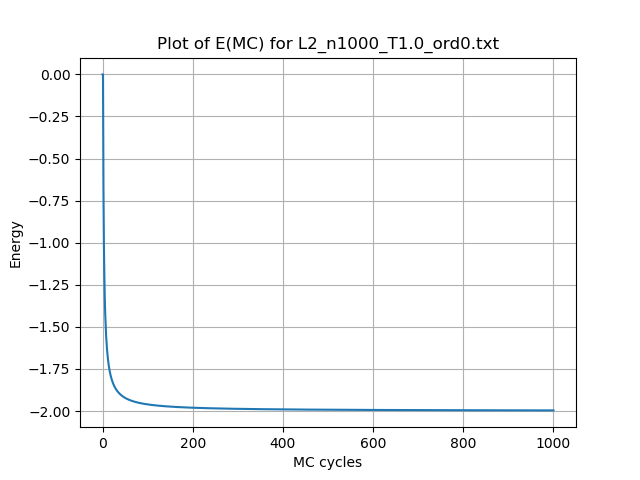
\includegraphics[width = 11cm]{img/energy_L2_n1000_T10_ord0.png}
      \caption{Energy-plot as function of MC-cycles. 2x2, MC1000, T=1.0, unordered spin}
      \label{fig:energy_L2_n1000_T1.0_ord0}
    \end{figure}

  \begin{figure}[ht]
      \centering
      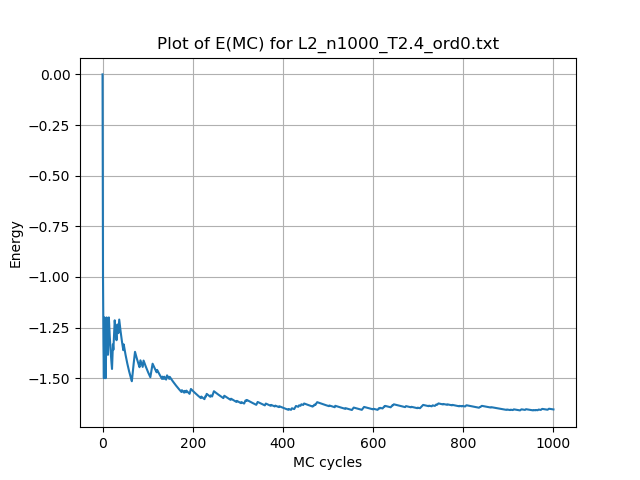
\includegraphics[width = 11cm]{img/energy_L2_n1000_T24_ord0.png}
      \caption{Energy-plot as function of MC-cycles. 2x2, MC1000, T=2.4, unordered spin}
      \label{fig:energy_L2_n1000_T2.4_ord0}
    \end{figure}

  \begin{figure}[ht]
      \centering
      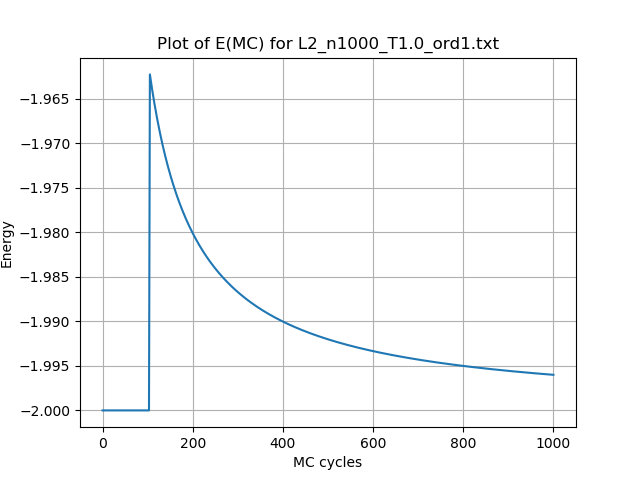
\includegraphics[width = 11cm]{img/energy_L2_n1000_T10_ord1.png}
      \caption{Energy-plot as function of MC-cycles. 2x2, MC1000, T=1.0, ordered spin}
      \label{fig:energy_L2_n1000_T1.0_ord1}
    \end{figure}

  \begin{figure}[ht]
      \centering
      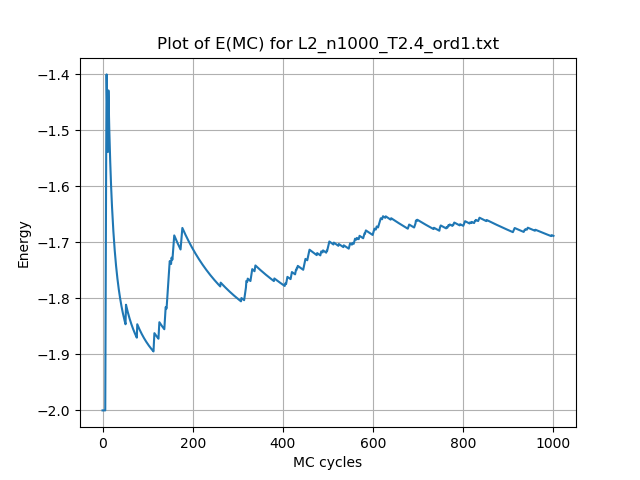
\includegraphics[width = 11cm]{img/energy_L2_n1000_T24_ord1.png}
      \caption{Energy-plot as function of MC-cycles. 2x2, MC1000, T=2.4, ordered spin}
      \label{fig:energy_L2_n1000_T2.4_ord1}
    \end{figure}

  \subsection{20x20-lattice}


  ????????????????????????????????????? \\
  ???????????????? \\


  \subsubsection{Acceptance}

  \begin{figure}[ht]
      \centering
      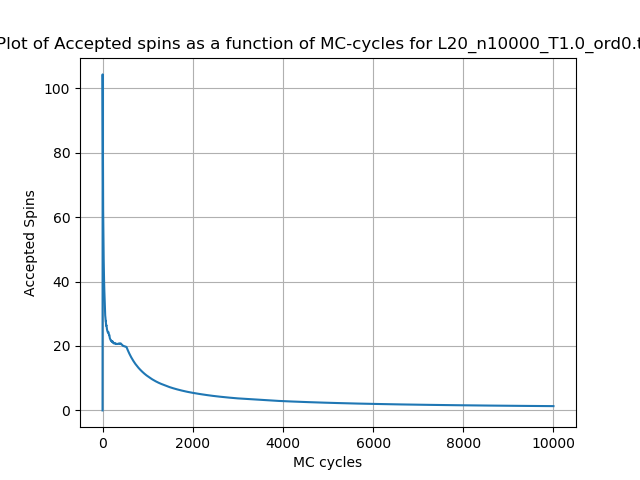
\includegraphics[width = 11cm]{img/accept_L20_n10000_T10_ord0.png}
      \caption{Cumulative acceptance per MC-cycle so far MC10000, T=1.0, unordered spin}
      \label{fig:accept_L20_n10000_T1.0_ord0}
    \end{figure}

  \begin{figure}[ht]
      \centering
      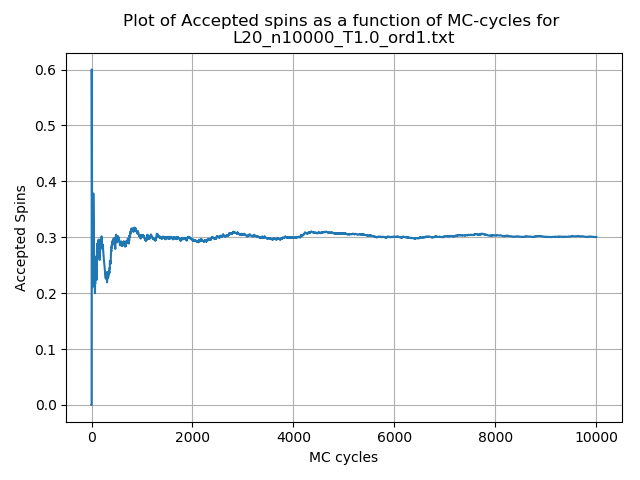
\includegraphics[width = 11cm]{img/accept_L20_n10000_T10_ord1.png}
      \caption{Cumulative acceptance per MC-cycle so far MC10000, T=1.0, ordered spin}
      \label{fig:accept_L20_n10000_T1.0_ord1}
    \end{figure}

  \begin{figure}[ht]
      \centering
      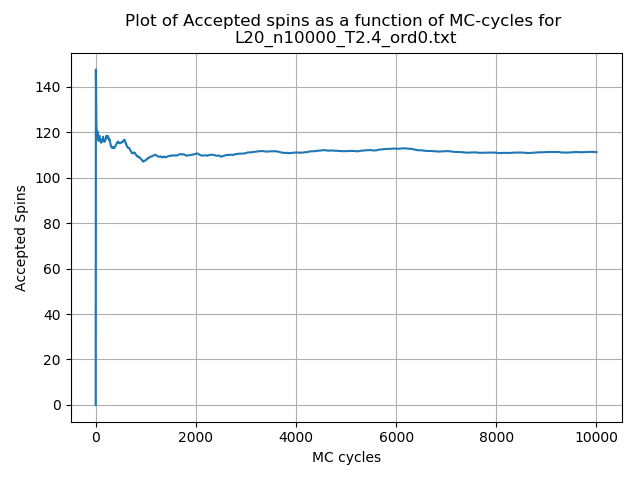
\includegraphics[width = 11cm]{img/accept_L20_n10000_T24_ord0.png}
      \caption{Cumulative acceptance per MC-cycle so far MC10000, T=2.4, ordered spin}
      \label{fig:accept_L20_n10000_T2.4_ord0}
    \end{figure}

  \begin{figure}[ht]
      \centering
      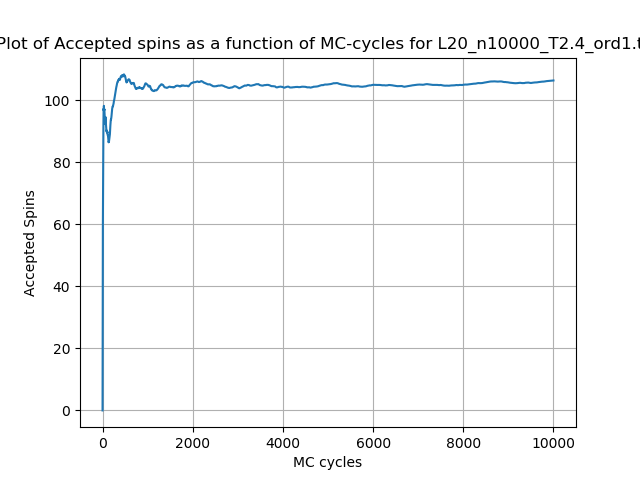
\includegraphics[width = 11cm]{img/accept_L20_n10000_T24_ord1.png}
      \caption{Cumulative acceptance per MC-cycle so far MC10000, T=2.4, ordered spin}
      \label{fig:accept_L20_n10000_T2.4_ord1}
    \end{figure}

  \subsubsection{Probability distributions}

  \begin{figure}[ht]
      \centering
      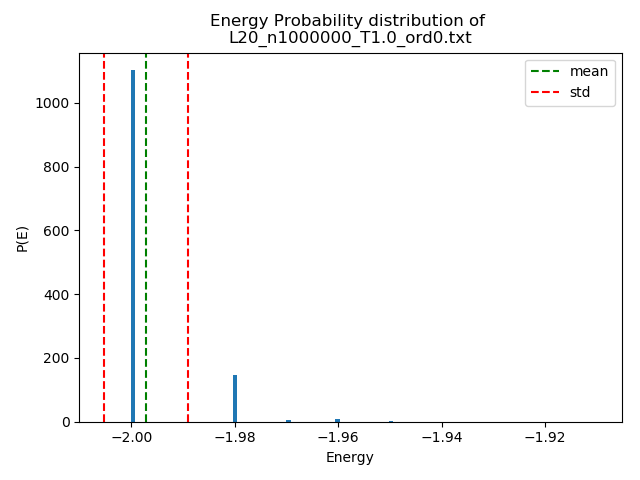
\includegraphics[width = 11cm]{img/energyhistogram_L20_n1000000_T10_ord0.png}
      \caption{Probability Distribution for low temperature with unordered spin (L=20, n=1mill)}
      \label{fig:prob-lowT-ord0}
    \end{figure}

  \begin{figure}[ht]
      \centering
      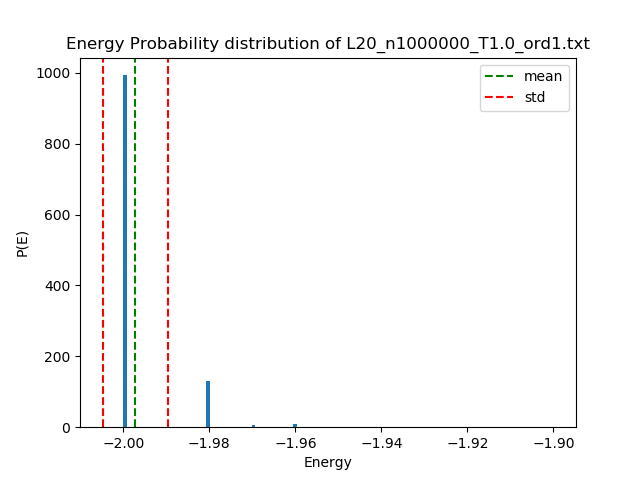
\includegraphics[width = 11cm]{img/energyhistogram_L20_n1000000_T10_ord1.png}
      \caption{Probability Distribution for low temperature with ordered spin (L=20, n=1mill)}
      \label{fig:prob-lowT-ord1}
    \end{figure}

  \begin{figure}[ht]
      \centering
      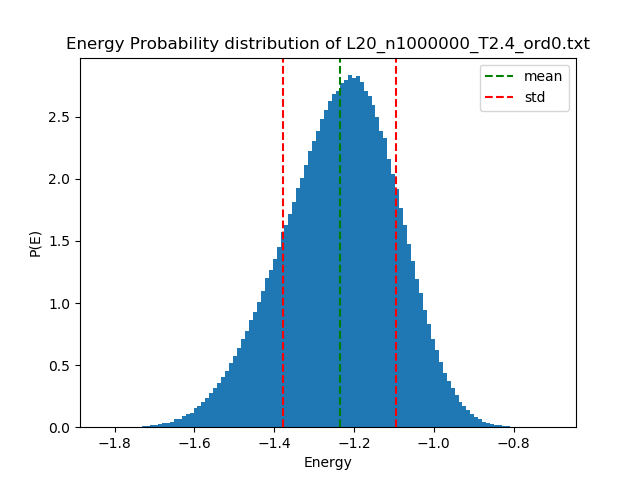
\includegraphics[width = 11cm]{img/energyhistogram_L20_n1000000_T24_ord0.png}
      \caption{Probability Distribution for high temperature with unordered spin (L=20, n=1mill)}
      \label{fig:prob-highT-ord0}
    \end{figure}

  \begin{figure}[ht]
      \centering
      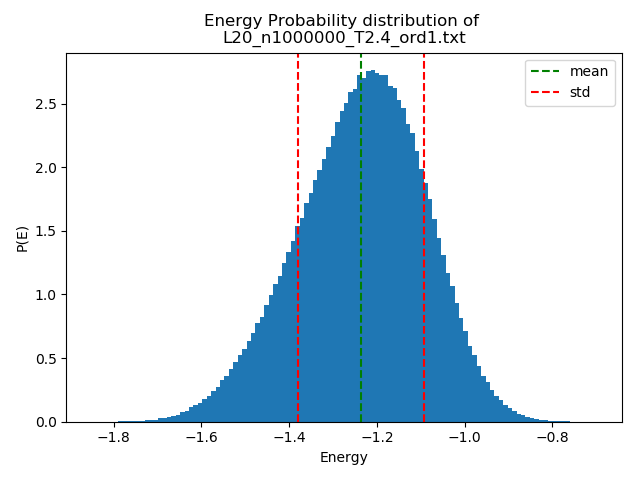
\includegraphics[width = 11cm]{img/energyhistogram_L20_n1000000_T24_ord1.png}
      \caption{Probability Distribution for high temperature with ordered spin (L=20, n=1mill)}
      \label{fig:prob-highT-ord1}
    \end{figure}

  \subsection{Critical Temperature}

  The critical temperature for the different simulations is as shown in table (\ref{tab:critical}).

    \begin{table}[ht]
      \centering
      \caption{Critical temperature for simulations}
      \vspace{2mm}
      \label{tab:critical2}
      \begin{tabular}{|c|c|}
          \hline
           L & $T_c$\\
          \hline \hline
          40 & 2.280 \\
          60 & 2.280 \\
          80 & 2.275 \\
          100 & 2.275 \\
          \hline
      \end{tabular} \\
      \hspace{0pt}\\
    \end{table}

  To avoid $a=0$, 100 will compare with 60 (case 1), and 80 with 40 (case 2).
  For case 1 the $a$-value is given as:
  $$(T_c(L_{100})-T_c(L_{60}))\cdot(L_{100}-L_{60})=a$$
  $$a=(2.275-2.280)\cdot(100-60)=-\frac{1}{5}=-0.2$$
  For case 2 $a$ will also be $-0.2$.

  $$T_c(L=\infty)=\frac{a}{L}-T_c(L)$$

  For case $L=100$:
  $$T_c(L=\infty)=\frac{-0.2}{100}-2.275$$

  Following the same structure for each L the following results are gotten. See table (\ref{tab:critical2})


    \begin{table}[ht]
      \centering
      \caption{Critical temperature using \cite{onsager}}
      \vspace{2mm}
      \label{tab:critical}
      \begin{tabular}{|c|c|}
          \hline
           L & $T_c(L=\infty)$\\
          \hline \hline
          40  & 2.2850 \\
          60  & 2.2833 \\
          80  & 2.2775 \\
          100 & 2.2770 \\
          onsager & 2.269 \\
          \hline
      \end{tabular} \\
      \hspace{0pt}\\
    \end{table}

%--------------- Discussion ---------------------------------------
\vspace{1cm}

\clearpage
\newpage

\section{Discussion} \label{sec:Discussion}

Comparing the \texorpdfstring{ $2 \times 2$ }{text}-lattice's numerical values with the analytical ones we see there is a major discrepancy. See table (\ref{tab:analyticalvsnumerical}). This is quite unnerving. However, after many hours of debugging and re-checking analytical expressions, no reason was found, and as such the results have been left like that. The reason for this error could be from numerical errors, truncation errors hidden somewhere, faulty expressions or other similar explanations.

For 4c) see RESULTS.txt

%------------------------------------------------------


\section{4c}
\subsection{results - må splitte dette i diskusjon og resultater}
In this section we will be looking at how many Monte Carlo cycles will be needed in order to reach an equilibrium state of the L = 20 system. This will be analyzed both for the energy of the system and the magnetization. First the T = 1 will be covered and later T = 2.4 as a comparison. The number of accepted spins as a function of Monte Carlo cycles will also be covered here.

PRESANTER GRAFENE HER start


magnet\_L20\_n1000000\_T24\_ord1.png

magnet\_L20\_n10000\_T10\_ord1.png

energy\_L20\_n1000000\_T10\_ord1.png

energy\_L20\_n10000\_T10\_ord1.png

PRESANTER GRAFENE HER slutt

Looking at the graphs for the energy states with 10.000 Monte Carlo cycles we can see that the energy states quite quickly reaches an equilibrium state. between 2000 and 4000 has an extremely little variance of less than 0.0005. With the value ranging from roughly -1.997 and -1.9968. To later flatten ought an roughly -1.997. Now looking at the system withe 1000.000 Monte Carlo cycles we see that the energy equilibrium at around 400.000 cycles. The energy value of the equilibrium state is roughly -1.99725. The difference between the 1000.000 and the 10.000 is therefore quite small. This shows that for the L=20 system it is more than enough with 10.000 Monte Carlo cycles for vary accurate data.

The same goes for the magnetisation. At 10.000 an equilibrium state is once again reached roughly at around 4000 cycles, with a magnetization value of roughly 0.99925. For the 1000.000 MC cycles magnetization plot, an equilibrium is observed just under 0.9993. This equilibrium lies roughly at 0.99927 magnetization.

Now magnetization and the energy for T = 2.4 will be discussed.

PRESANTER GRAFENE HER start

magnet\_L20\_n10000\_T24\_ord1.png
magnet\_L20\_n1000000\_T24\_ord1.png

energy\_L20\_n10000\_T24\_ord1.png
energy\_L20\_n1000000\_T24\_ord1.png

PRESANTER GRAFENE HER slutt

For the energies more or less the same result will be reached for 10.000 MC cycles as for 1000.000 cycles. As one can see from the graphs above. They both flatten ought at the roughly energy of -1.26. Unless extreme precision is needed 10.000 MC cycles should be enough to find the energy equilibrium state. \\

However this is not true for the magnetization. For 10.000 MC cycles there is no real equilibrium stat reached that is observable. How ever once one comperes it to the 1000.000 MC cycle run one can observe that equilibrium is reached at about 400.000 MC cycles. \\


accept\_L2\_n1000\_T24\_ord1.png

%----------------------------------------------------------


For 4d) Jeg prøvde SÅ HARDT å fikse et plot av sannsynlighetsfordelingen, men det ble f*cked
Se koden for hva jeg har gjort og prøv å finne ut av det.
I PDF-en for Project 4 står det vi skal sammenligne med variansen.. prøv å fikse
i koden prøvde jeg å bruke variansen som filter, men tror ikke vi kan det. Samtidig må vi kutte ut all dataen som lages før latticen når equilibrium. \\

Looking at the probability distributions for L=20 we found them pretty sensible at higher temperatures. For low temperatures they did not look very good. This is most likely attributed to the fact that low temperatures makes the metropolis algorithm less likely to accept a spin-flip, leading to fewer changes. The energies are more stable and as such only a few peaks exist. See figures (\ref{fig:accept_L20_n10000_T1.0_ord0}) - (\ref{fig:accept_L20_n10000_T2.4_ord1}). \\


%--------------------------------------------------------


For 4e) ALEXANDRA \\

Looking at the final plots comparing the different L-values' heat-capacity an indication of a phase transition can be found. There is a large change in the data observed around $T=2.25$, and this would be due to a change in the structure, a phase transition. \\

{\Huge ALEXANDRA HER MÅ DU REFERERE TIl PLOTTENE MED L=40,60,80,100 \par}


%----------------------------------------------------------


For 4f) ERIK \\

Studying the critical temperature we found the results to be resonable. Due to a fixed step-length L40 and L60 had the same estimated $T_c$. The same went for L80 and L100. This was interesting, but not unlikely. One would think that increasing the lattice by that much would change the result, but it was pretty close. Had the results been smoothed out with least squares or something of the sort, a different number would have been found. However, this could easily be less accurate. When using \cite{task}'s Eq. (3), and calculating the $a$-value the final results were made. See table (\ref{tab:critical2}). \\

L100 was the closest, as it should and was 0.008 higher than Onsager's result was \cite{onsager}. This is pretty good.
Though increasing the lattice size further would lead to extremly slow calculations, we assume this would quickly converge to Onsager's value. \\


%---------------Conclusion and perspective---------------------------
\vspace{1cm}

\section{Conclusion and perspective} \label{sec:Conclusion}

In this project we have studied, among many other things, the number of Monte Carlo cycles needed to reach an equilibrium state. Based on the data acquired the number of cycles needed to reach an equilibrium state with a two decimal accuracy would be 6000 MC cycles for the temperatures tested in this project. This should allow enough cycles for the system to clearly have stabilised. For the magnetization however it seams to bee a need for more cycles. Somewhere around 400.000 cycles in order to be curtain regardless of temperature. This was how ever not the case for the T=1 \\


%----------------References----------------------------------------

\vspace{1cm}

\section{References} \label{sec:References}

\begin{thebibliography}{}

\bibitem{task}
Morten H. Jensen (2019), \href{https://github.com/CompPhysics/ComputationalPhysics/blob/master/doc/Projects/2019/Project4/pdf/Project4.pdf}{Project 4}, Departement of Physics, University of Oslo, Norway

\bibitem{github}
Erik B. Grammeltvedt, Alexandra Jahr Kolstad, Erlend T. North (2019), \href{https://github.com/Erikbgram/Fys3150}{GitHub}, Students of Departement of Physics, University of Oslo, Norway

\bibitem{lecture_slides}
Morten H. Jensen (2015), \href{https://github.com/CompPhysics/ComputationalPhysics/blob/master/doc/Lectures/lectures2015.pdf}{Lecture slides for FYS3150}, Department of Physics, University of Oslo, Norway

\bibitem{onsager}
Onsager (1944), \href{https://journals.aps.org/pr/abstract/10.1103/PhysRev.65.117}{"A Two-Dimensional Model with an Order-Disorder Transition"}, American Physical Society

\bibitem{isingmodel}
Jacob Linder (2018), \href{https://snl.no/Ising-modellen}{Ising-modellen}, Store Norske Leksikon \\

\end{thebibliography}


%--------------Appendix---------------------------------------------
\vspace{1cm}


\appendix
\section{Appendix - endre navn senere?} \label{sec:Appendix}


\subsection{Derivation of analytical formulae}

To derive the analytical formulae we need to know the hyperbolic functions cosh and sinh, and their correlation to the exponential function. \\

They are as follows

\begin{align*}
    2 \cosh (x) &= e^x + e^{-x} \\
    2 \sinh (x) &= e^x - e^{-x}
\end{align*} \\


\subsubsection{Derivation of the partition function} \label{sec:derivationpartitionfunction}

The partition function is introduced in section \ref{sec:partitionfunction}. \\

Deriving the equation.

\begin{align*}
  Z &= \sum_{i=1} ^{M} e^{- \beta E_i} = \sum_{i=1} ^{16} e^{- \beta E_i} \\
  &= 1 \cdot e^{- \beta (-8J)} + 4 \cdot e^{- \beta (0J)} + 2 \cdot e^{- \beta (8J)} + 4 \cdot e^{- \beta (0J)}
  + 4 \cdot e^{- \beta (0J)} + 1 \cdot e^{- \beta (-8J)} \\
  &= e^{8 \beta J} + 4 + 2 \cdot e^{-8 \beta J} + 4 + 4 + e^{8 \beta J} \\
  &= 2 e^{8 \beta J } + 2 e^{-8 \beta J} + 12 \\
  &= 2 \left( e^{8 \beta J} + e^{- 8 \beta J} \right) + 12 \\
  &= 2 \left( 2 \cosh(8 \beta J) \right) + 12 \\
  &= 4 \cosh(8 \beta J) + 12
\end{align*} \\


\subsubsection{Derivation of the expectation values of the energies} \label{sec:derivationenergies}

The expectation value of the energy is introduced in section \ref{sec:energyandmagnetization}. \\

Deriving the equation.

\begin{align*}
  \langle E \rangle &= \frac{1}{Z} \sum _{i=1} ^M E_i e^{- \beta E_i} \\
  &= \frac{1}{Z} \left[ 1 \cdot (-8J) e^{- \beta (-8J)} + 4 \cdot 0 + 2 \cdot (8J) e^{- \beta (8J)} + 4 \cdot 0 + 1 \cdot (-8J) e^{- \beta (-8J)} \right] \\
  &= \frac{1}{Z} \left[ - 8J e^{\beta 8J} + 2 \cdot 8J e^{- \beta 8J} - 8J e^{ \beta 8J} \right] \\
  &= \frac{2}{Z} \left[ - 8J e^{\beta 8 J} + 8 J e^{- \beta 8 J} \right] \\
  &= - \frac{16 J}{Z} \left( e^{8 \beta J} - e^{- 8 \beta J} \right) \\
  &= - \frac{16 J}{Z} (2 \sinh(8 \beta J) ) \\
  &= - \frac{32 J}{Z} \sinh(8 \beta J)
\end{align*} \\

The expectation value of the energy squared is introduced in section \ref{sec:specificheat}. \\

Deriving the equation.

\begin{align*}
  \langle E^2 \rangle &= \frac{1}{Z} \sum _{i=1} ^M E_i^2 e^{- \beta E_i} \\
  &= \frac{1}{Z} \left[ 1 \cdot (-8J)^2 e^{- \beta (-8J)} + 4 \cdot 0 + 2 \cdot (8J)^2 e^{- \beta (8J)} + 4 \cdot 0 + 1 \cdot (-8J)^2 e^{- \beta (-8J)} \right] \\
  &= \frac{1}{Z} \left[ 64 J^2 e^{\beta 8J} + 2 \cdot 64 J^2 e^{- \beta 8J} + 64 J^2 e^{ \beta 8J} \right] \\
  &= \frac{2 \cdot 64 J^2}{Z} \left[ e^{\beta 8 J} + e^{- \beta 8 J} \right] \\
  &= \frac{128 J^2}{Z} (2 \cosh(8 \beta J) ) \\
  &= \frac{256 J^2}{Z} \cosh(8 \beta J)
\end{align*} \\


\subsubsection{Derivation of the expectation values of the magnetizations} \label{sec:derivationmagnetizations}

The expectation value of the magnetization is introduced in section \ref{sec:energyandmagnetization}. \\

Deriving the equation.

\begin{align*}
  \langle \mathcal{M} \rangle &= \frac{1}{Z} \sum _{i=1} ^M \mathcal{M}_i e^{- \beta E_i} \\
  &= \frac{1}{Z} \left[1 \cdot 4 e^{- \beta (-8J)} + 4 \cdot 2 e^{- \beta (0J)} + 2 \cdot 0 + 4 \cdot 0 + 4 \cdot (-2)
  e^{- \beta (0J)} + 1 \cdot (-4) e^{- \beta (-8J)} \right] \\
  &= \frac{1}{Z} \left[ 4 e^{\beta 8J} + 8 - 8 - 4 e^{ \beta 8J} \right] \\
  &= \frac{1}{Z} \cdot 0 \\
  &= 0
\end{align*} \\

The expectation value of the mean magnetization is introduced in section \ref{sec:energyandmagnetization}. \\

Deriving the equation.

\begin{align*}
    \langle | \mathcal{M} | \rangle &= \frac{1}{Z} \sum _{i=1} ^M |\mathcal{M}_i| e^{- \beta E_i} \\
    &= \frac{1}{Z} \left[1 \cdot |4| e^{- \beta (-8J)} + 4 \cdot |2| e^{- \beta (0J)} + 2 \cdot |0| + 4 \cdot |0| + 4 \cdot |-2|
    e^{- \beta (0J)} + 1 \cdot |-4| e^{- \beta (-8J)} \right] \\
    &= \frac{1}{Z} \left[ 4 e^{\beta 8J} + 8 + 8 + 4 e^{ \beta 8J} \right] \\
    &= \frac{1}{Z} \cdot 4 \left[ 2 e^{\beta 8J} + 4 \right] \\
    &= \frac{8}{Z} \left( e^{\beta 8J} + 2 \right) \\
\end{align*}

The expectation value of the magnetization squared is introduced in section \ref{sec:susceptibility}. \\

Deriving the equation.

\begin{align*}
  \langle \mathcal{M}^2 \rangle &= \frac{1}{Z} \sum _{i=1} ^M \mathcal{M}_i^2 e^{- \beta E_i} \\
  &= \frac{1}{Z} \left[1 \cdot 4^2 e^{- \beta (-8J)} + 4 \cdot 2^2 e^{- \beta (0J)} + 2 \cdot 0 + 4 \cdot 0 + 4 \cdot (-2)^2 e^{- \beta (0J)} + 1 \cdot (-4)^2 e^{- \beta (-8J)} \right] \\
  &= \frac{1}{Z} \left[ 16 e^{\beta 8J} + 16 + 16 + 16 e^{ \beta 8J} \right] \\
  &= \frac{1}{Z} \left[ 2 e^{8 \beta J} + 2 \right] \\
  &= \frac{32}{Z} \left( e^{8 \beta J} + 1 \right) \\
\end{align*}


\subsection{Extracting the critical temperature} ??????????????????????

In order to find the critical temperature we will use \cite{task}'s Eq. (3). It is shown below:
$$T_c(L)-T_c(L=\infty)=aL^{-1/\nu}$$
where $\nu=1$. This gives
$$T_c(L)-T_c(L=\infty)=\frac{a}{L}$$
In order to find $a$ we subtract the equation with different $L$-values.
$$T_c(L_{100})-T_c(L=\infty)=\frac{a}{L_{100}}$$
$$T_c(L_{80})-T_c(L=\infty)=\frac{a}{L_{80}}$$
Subtracting gives
$$T_c(L_{100})-T_c(L_{80})=\frac{a}{L_{100}-L_{80}}$$
$$(T_c(L_{100})-T_c(L_{80}))\cdot(L_{100}-L_{80})=a$$ \label{eq:finding-a}

%\clearpage



%----------------Slutten av dokumentet---------------------------------------


%\end{multicols}

\end{document}
